\documentclass[arhiv]{izpit}
\usepackage{fouriernc}
\usepackage{tikz}

\begin{document}

\izpit{Programiranje I: 1.\ izpit}{6.\ februar 2011}{
  Čas reševanja je 150 minut.
  Doseženih 100 točk šteje za maksimalno oceno.
  Veliko uspeha!
}

%%%%%%%%%%%%%%%%%%%%%%%%%%%%%%%%%%%%%%%%%%%%%%%%%%%%%%%%%%%%%%%%%%%%%%
\naloga[35 točk]

Stanje na bančnih računih oseb predstavimo s slovarjem, ki ime računa preslika v trenutno
stanje na računu, na primer:
%
{\small\begin{verbatim}
   {'Ana': 5, 'Bine': 120, 'Cene': 310, 'Darko': 42}
\end{verbatim}}\noindent
%
Prenos med računoma je urejena trojica $(A, B, X)$, ki pomeni, da iz računa $A$ na
račun $B$ prenesemo $X$.

\podnaloga[15 točk]
Sestavite funkcijo \verb|naloga1a(s, p)|, ki sprejme stanje \verb|s| na bančnih računih in seznam prenosov \verb|p| ter osveži stanje. Na primer
%
{\small\begin{verbatim}
   >>> s = {'Ana': 5, 'Bine': 120, 'Cene': 310, 'Darko': 42}
   >>> naloga1a(s, [('Ana', 'Bine', 10), ('Bine', 'Cene', 50), ('Cene', 'Bine', 10)])
   >>> s
   {'Ana': -5, 'Bine': 90, 'Cene': 350, 'Darko': 42}
\end{verbatim}}

\podnaloga[20 točk]
Sestavite funkcijo \verb|naloga1b(s1, s2)|, ki sprejme dve stanji in vrne seznam prenosov, s katerim iz \verb|s1| dobimo \verb|s2|. Predpostaviti smete, da imata \verb|s1| in \verb|s2| enake ključe. Funkcija naj vrne \verb|None|, če tak seznam prenosov ne obstaja.
Primer:
%
{\small\begin{verbatim}
   >>> naloga1b({'Ana': 10, 'Bine': 20, 'Cene': 40}, {'Ana': 20, 'Bine': 25, 'Cene': 25})
   [('Cene', 'Bine', 5), ('Cene', 'Ana', 10)]
\end{verbatim}}

% def naloga1a(stanje, prenosi):
%     for (a, b, x) in prenosi:
%         stanje[a] -= x
%         stanje[b] += x

% def naloga1b(s1, s2):
%     racuni = list(s1.keys())
%     prenosi = []
%     if not racuni:
%         return []
%     else:
%         a = racuni.pop() # Tega uporabimo kot banko
%         k = s2[a] - s1[a]
%         for b in racuni:
%             x = s2[b] - s1[b]
%             if x > 0: prenosi.append((a, b, x))
%             elif x < 0: prenosi.append((b, a, -x))
%             k += x
%         return (prenosi if k == 0 else None)


%%%%%%%%%%%%%%%%%%%%%%%%%%%%%%%%%%%%%%%%%%%%%%%%%%%%%%%%%%%%%%%%%%%%%%
\naloga[25 točk]

Pot v iskalnem drevesu lahko predstavimo s seznamom vrednosti \verb|True| in \verb|False|.
Vrednost \verb|True| pove, da naredimo korak v levo poddrevo, vrednost \verb|False| pa, da ga naredimo v desno poddrevo.
Tako v drevesu
\[
  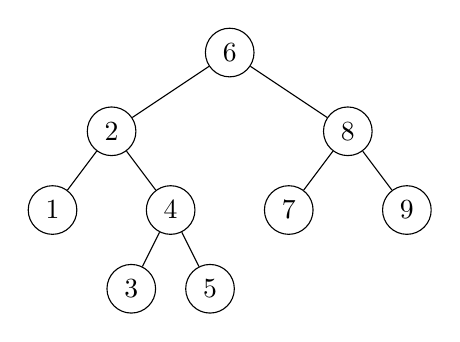
\begin{tikzpicture}[level distance=1cm,
    level 1/.style={sibling distance=3cm},
    level 2/.style={sibling distance=1.5cm},
    level 3/.style={sibling distance=1cm}
    ]
    \node[circle, draw] {6}
      child {node[circle, draw] {2}
        child {node[circle, draw] {1}}
        child {node[circle, draw] {4}
          child {node[circle, draw] {3}}
          child {node[circle, draw] {5}}
        }
      }
      child {node[circle, draw] {8}
      child {node[circle, draw] {7}}
        child {node[circle, draw] {9}}
      };
  \end{tikzpicture}
\]
seznam \verb|[True, False, True]| predstavlja pot do \verb|3|,
seznam \verb|[False]| pot do \verb|8|,
seznam \verb|[]| pot do korena \verb|6|,
seznam \verb|[False, False, True]| pa ne predstavlja poti v drevesu.

\podnaloga[10 točk]
%
Razredu \verb|IskalnoDrevo| dodajte metodo \verb|naloga2a(self, p)|, ki vrne element v danem drevesu, do katerega pridemo s potjo \verb|p|.
Če v drevesu take poti ni, naj metoda vrne \verb|None|.

% def naloga2a(self, p):
%     if self.prazno:
%         return None
%     elif pot:
%         smer = p.pop(0)
%         if smer:
%             return self.levo.naloga2a(p)
%         else:
%             return self.desno.naloga2a(p)
%     else:
%         return self.vrednost

\podnaloga[15 točk]
%
Razredu \verb|IskalnoDrevo| dodajte metodo \verb|naloga2b(self, x)|, ki vrne seznam,
ki predstavlja pot do elementa \verb|x|.
Če v drevesu danega elementa ni, naj metoda vrne \verb|None|.

% def naloga2b(self, x):
%     if self.prazno:
%         return None
%     elif self.vrednost == x:
%         return []
%     elif self.vrednost < x:
%         leva_pot = self.levo.naloga2b(x)
%         if leva_pot: return [True] + leva_pot
%     else:
%         desna_pot = self.desno.naloga2b(x)
%         if desna_pot: return [False] + desna_pot

%%%%%%%%%%%%%%%%%%%%%%%%%%%%%%%%%%%%%%%%%%%%%%%%%%%%%%%%%%%%%%%%%%%%%%
\naloga[25 točk]

V Mathematici sestavite funkcijo \verb|naloga3[z_, v_]|, ki sprejme zmagovalno kombinacijo \verb|z|, izžrebano na Lotu, ter seznam \verb|v| vplačanih kombinacij. Funkcija vrne število posameznih zadetkov, torej koliko štiric, petic, šestic in sedmic je bilo vplačanih. Dobitka $6 + 1$, Lotka in ostalih nagrad ne upoštevamo. Na primer:
%
{\small\begin{verbatim}
   In[1]:= naloga3[{14, 16, 19, 20, 27, 31, 38}, {
                   {14, 16, 19, 20, 26, 31, 35},
                   {14, 16, 19, 20, 27, 30, 38},
                   {14, 16, 19, 20, 26, 30, 37},
                   {10, 14, 18, 22, 26, 30, 34},
                   {14, 16, 19, 20, 27, 31, 38},
                   {14, 16, 19, 20, 27, 30, 37}}]
   Out[1]= {{5, 2}, {6, 1}, {4, 1}, {7, 1}}
   In[2]:= naloga3[{14, 16, 19, 20, 27, 31, 38}, {
                   {38, 31, 27, 20, 19, 16, 14},
                   {10, 14, 18, 22, 26, 30, 34}}]
   Out[2]= {{7, 1}}\end{verbatim}}
%
\noindent \textbf{Namig:} Oglejte si, kaj počne funkcija \verb|Tally|.

% naloga3[z_, v_] := Tally[Select[
%     Map[Function[komb, Length[Intersection[komb, z]]], v],
%     Function[dobitek, dobitek > 3]
%   ]]


%%%%%%%%%%%%%%%%%%%%%%%%%%%%%%%%%%%%%%%%%%%%%%%%%%%%%%%%%%%%%%%%%%%%%%
\naloga[25 točk]

\emph{Transpozicija} v tabeli \verb|t| je zamenjava dveh elementov. Transpozicijo, ki zamenja \verb|t[i]| in \verb|t[j]| predstavimo z urejenim parom \verb|(i, j)|.
Sestavite funkcijo \verb|naloga4(t)|, ki vrne seznam transpozicij, s katerimi uredimo dano tabelo \verb|t|. Na primer
%
{\small\begin{verbatim}
   >>> naloga4([9, 7, 5, 3])
   [(0, 3), (1, 2)]
   >>> naloga4([3, 5, 7, 9])
   []
\end{verbatim}}

%def naloga4(t):
%    t = t[:]
%    p = []
%    for i in range(0, len(t) - 1):
%        j = i
%        for k in range(i + 1, len(t)):
%            if t[k] < t[j]: j = k
%        (t[i],t[j]) = (t[j], t[i])
%        if i != j: p.append((i,j))
%    return p


\end{document}

